
\chapter{El camino hacia el programa}

El objetivo de este libro es el de enseñar al estudiante a pensar
como lo hacen los científicos informáticos. Esta manera de pensar
combina las mejores características de la matemática, la ingeniería
y las ciencias naturales. Como los matemáticos, los científicos informáticos
usan lenguajes formales para diseñar ideas (específicamente, cómputos).
Como los ingenieros, ellos diseñan cosas, construyendo sistemas mediante
el ensamble de componentes y evaluando las ventajas y desventajas
de cada una de las alternativas de construcción. Como los científicos,
ellos observan el comportamiento de sistemas complejos, forman hipótesis,
y prueban sus predicciones.

La habilidad más importante del científico informático es \textbf{la
solución de problemas}. La solución de problemas incluye poder formular
problemas, pensar en soluciones de manera creativa y expresar soluciones
clara y precisamente. Como se verá, el proceso de aprender a programar
es la oportunidad perfecta para desarrollar la habilidad de resolver
problemas. Por esa razón este capítulo se llama ``El camino hacia
el programa''.

A cierto nivel, usted aprenderá a programar, lo cual es una habilidad
muy útil por sí misma. A otro nivel, usted utilizará la programación
para obtener algún resultado. Ese resultado se verá más claramente
durante el proceso.

\section{El lenguaje de programación Python}

\index{lenguaje de programación} \index{lenguaje!programación}

El lenguaje de programación que aprenderá es Python. Python es un
ejemplo de \textbf{lenguaje de alto nivel}; otros ejemplos de lenguajes
de alto nivel son C, C++, Perl y Java.

Como se puede deducir de la nomenclatura ``lenguaje de alto nivel,''
también existen \textbf{lenguajes de bajo nivel}, que también se denominan
lenguajes de máquina o lenguajes ensambladores. A propósito, las computadoras
sólo ejecutan programas escritos en lenguajes de bajo nivel. Los programas
de alto nivel tienen que ser traducidos antes de ser ejecutados. Esta
traducción lleva tiempo, lo cual es una pequeña desventaja de los
lenguajes de alto nivel.

\index{portátil} \index{lenguaje de alto nivel} \index{lenguaje de bajo nivel}
\index{lenguaje!alto nivel} \index{lenguaje!bajo nivel}

Aun así, las ventajas son enormes. En primer lugar, la programación
en lenguajes de alto nivel es mucho más fácil; escribir programas
en un lenguaje de alto nivel toma menos tiempo ya que los programas
son más cortos, más fáciles de leer, y es más probable que queden
correctos. En segundo lugar, los lenguajes de alto nivel son \textbf{portables},
lo que significa que los programas escritos con estos pueden ser ejecutados
en tipos diferentes de computadoras sin modificación alguna o con
pocas modificaciones. Programas escritos en lenguajes de bajo nivel
sólo pueden ser ejecutados en un tipo de computadora y deben ser reescritos
para ser ejecutados en otra.

Debido a estas ventajas, casi todo programa se escribe en un lenguaje
de alto nivel. Los lenguajes de bajo nivel son sólo usados para unas
pocas aplicaciones especiales.

\index{compilar} \index{interpretar}

Hay dos tipos de programas que traducen lenguajes de alto nivel a
lenguajes de bajo nivel: \textbf{intérpretes} y \textbf{compiladores}.
Un intérprete lee un programa de alto nivel y lo ejecuta, lo que significa
que lleva a cabo lo que indica el programa. Traduce el programa poco
a poco, leyendo y ejecutando cada comando.

\vspace{0.1in}
 \centerline{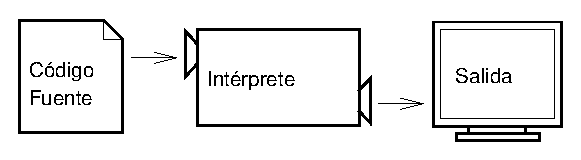
\includegraphics[scale=0.7]{illustrations/interpret}}
\vspace{0.1in}

Un compilador lee el programa y lo traduce todo al mismo tiempo, antes
de ejecutar alguno de los programas. A menudo se compila un programa
como un paso aparte, y luego se ejecuta el código compilado. En este
caso, al programa de alto nivel se lo llama el \textbf{código fuente},
y al programa traducido es llamado el \textbf{código de objeto} o
el \textbf{código ejecutable}.

\vspace{0.1in}
 \centerline{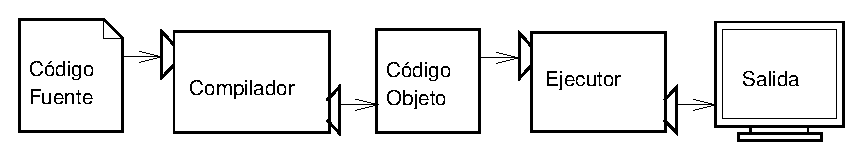
\includegraphics[scale=0.7]{illustrations/compile}}
\vspace{0.1in}

A Python se lo considera un lenguaje interpretado, porque sus programas
son ejecutados por un intérprete. Existen dos maneras de usar el intérprete:
modo de comando y modo de guión. En modo de comando se escriben sentencias
en el lenguaje Python y el intérprete muestra el resultado.
\begin{pyconcode}
$python
Python 3.6.1 (default, Apr 29 2017, 15:32:44) [GCC 5.4.0] on linux 
Type "help", "copyright", "credits" or "license" for more information. 
>>>1+1
2
\end{pyconcode}
La primera línea de este ejemplo es el comando que pone en marcha
al intérprete de Python. Las dos líneas siguientes son mensajes del
intérprete. La tercera línea comienza con {\verb+>>>+}, lo que
indica que el intérprete está listo para recibir comandos. Escribimos
\texttt{1+1} y el intérprete contestó \texttt{2}.

Alternativamente, se puede escribir el programa en un archivo y usar
el intérprete para ejecutar el contenido de dicho archivo. El archivo,
en este caso, se denomina un \textbf{guión (script)}; por ejemplo,
en un editor de texto se puede crear un archivo \texttt{unomasuno.py}
que contenga esta línea:

\begin{pyconcode}
print(1 + 1)
\end{pyconcode}

Por acuerdo unánime, los archivos que contienen programas de Python
tienen nombres que terminan con \texttt{.py}. Para ejecutar el programa,
se le tiene que indicar el nombre del guión al intérprete.

\begin{pyconcode}
$ python unomasuno.py
2
\end{pyconcode}
\begin{pyconcode}

\end{pyconcode}
En otros entornos de desarrollo, los detalles de la ejecución de programas
diferirán. Además, la mayoría de programas son más interesantes que
el anterior.

La mayoría de ejemplos en este libro son ejecutados en la línea de
comandos. La línea de comandos es más conveniente para el desarrollo
de programas y para pruebas rápidas, porque las instrucciones de Python
se pueden pasar a la máquina para ser ejecutadas inmediatamente. Una
vez que el programa está completo, se lo puede archivar en un guión
para ejecutarlo o modificarlo en el futuro.

\section{¿Qué es un programa?}

Un programa es una secuencia de instrucciones que especifican cómo
ejecutar un cómputo. El cómputo puede ser matemático, cómo solucionar
un sistema de ecuaciones o determinar las raíces de un polinomio,
pero también puede ser simbólico, cómo buscar y reemplazar el texto
de un documento o (aunque parezca raro) compilar un programa.

\index{instrucción}

Las instrucciones (comandos, órdenes) tienen una apariencia diferente
en lenguajes de programación diferentes, pero existen algunas funciones
básicas que se presentan en casi todo lenguaje:
\begin{description}
\item [{Entrada:}] recibir datos del teclado, o de un archivo o de otro
aparato.
\item [{Salida:}] mostrar datos en el monitor o enviar datos a un archivo
u otro aparato.
\item [{Matemáticas:}] ejecutar operaciones básicas, como la adición y
la multiplicación.
\item [{Operación condicional:}] probar la veracidad de alguna condición
y ejecutar una secuencia de instrucciones apropiada.
\item [{Repetición}] ejecutar alguna acción repetidas veces, usualmente
con alguna variación.
\end{description}
Aunque sea difícil de creer, todos los programas en existencia son
formulados exclusivamente con tales instrucciones. Así, una manera
de describir la programación es: el proceso de romper una tarea en
tareas cada vez más pequeñas hasta que éstas sean lo suficientemente
sencillas como para ser ejecutadas con una secuencia de estas instrucciones
básicas.

Quizás esta descripción es un poco ambigua. No se preocupe. Explicaremos
ésto con más detalle en el tema de \textbf{algoritmos}.

\section{¿Qué es la depuración (debugging)?}

\index{depuración (debugging)} \index{error (bug)}

La programación es un proceso complejo, y a veces este proceso lleva
a \textbf{errores indefinidos}, también llamados \textbf{defectos}
o \textbf{errores de programación} (en inglés `bugs'), y el proceso
de buscarlos y corregirlos es llamado \textbf{depuración} (en inglés
`debugging').

Hay tres tipos de errores que pueden ocurrir en un programa. Es muy
útil distinguirlos para encontrarlos más rápido.

\subsection{Errores sintácticos}

\index{error sintáctico} \index{error!sintaxis}

Python sólo puede ejecutar un programa si está sintácticamente bien
escrito. Al contrario, es decir, si el programa tiene algún error
de sintaxis, el proceso falla y devuelve un mensaje de error. La palabra
\textbf{sintáctica} se refiere a la estructura de cualquier programa
y a las reglas de esa estructura. \index{sintáctica} Por ejemplo,
en español, la primera letra de toda oración debe ser mayúscula y
el fin de toda oración debe llevar un punto. esta oración tiene un
error sintáctico. Esta oración también

Para la mayoría de lectores, unos pocos errores no impiden la comprensión
de los grafitis en la calle que, a menudo, rompen muchas reglas de
sintaxis. Sin embargo Python no es así. Si hay aunque sea un error
sintáctico en el programa, Python mostrará un mensaje de error y abortará
su ejecución. Al principio usted pasará mucho tiempo buscando errores
sintácticos, pero con el tiempo no cometerá tantos errores y los encontrará
rápidamente.

\subsection{Errores en tiempo de ejecución}

\label{runtime} \index{error en tiempo de ejecución} \index{error!en tiempo de ejecución}
\index{excepción} \index{lenguaje seguro} \index{seguro!lenguaje}

El segundo tipo de error es el de tiempo de ejecución. Este error
aparece sólo cuando se ejecuta un programa. Estos errores también
se llaman \textbf{excepciones}, porque indican que algo excepcional
ha ocurrido.

Con los programas que vamos a escribir al principio, los errores de
tiempo de ejecución ocurrirán con poca frecuencia.

\subsection{Errores semánticos}

\index{semántica} \index{error semántico} \index{semántico!error}

El tercer tipo de error es el \textbf{semántico}. Si hay un error
de lógica en su programa, éste será ejecutado sin ningún mensaje de
error, pero el resultado no será el deseado. El programa ejecutará
la lógica que usted le dijo que ejecutara.

A veces ocurre que el programa escrito no es el que se tenía en mente.
El sentido o significado del programa no es correcto. Es difícil hallar
errores de lógica. Eso requiere trabajar al revés, comenzando a analizar
la salida para encontrar al problema.

\subsection{Depuración experimental}

Una de las técnicas más importantes que usted aprenderá es la depuración.
Aunque a veces es frustrante, la depuración es una de las partes de
la programación más estimulantes, interesantes e intelectualmente
exigentes.

La depuración es una actividad parecida a la tarea de un investigador:
se tienen que estudiar las pistas para inferir los procesos y eventos
que han generado los resultados encontrados.

La depuración también es una ciencia experimental. Una vez que se
tiene conciencia de un error, se modifica el programa y se intenta
nuevamente. Si la hipótesis fue la correcta se pueden predecir los
resultados de la modificación y estaremos más cerca a un programa
correcto. Si la hipótesis fue la errónea tendrá que idearse otra hipótesis.
Como dijo Sherlock Holmes: ``Cuando se ha descartado lo imposible,
lo que queda, no importa cuan inverosímil, debe ser la verdad'' (A.
Conan Doyle, {\em The Sign of Four})

\index{Holmes, Sherlock} \index{Doyle, Arthur Conan}

Para algunas personas, la programación y la depuración son lo mismo:
la programación es el proceso de depurar un programa gradualmente,
hasta que el programa tenga el resultado deseado. Esto quiere decir
que el programa debe ser, desde un principio, un programa que funcione,
aunque su función sea solo mínima. El programa es depurado mientras
crece y se desarrolla.

Por ejemplo, aunque el sistema operativo Linux contenga miles de líneas
de instrucciones, Linus Torvalds lo comenzó como un programa para
explorar el microprocesador Intel 80836. Según Larry Greenfield: ``Uno
de los proyectos tempranos de Linus fue un programa que intercambiaría
la impresión de AAAA con BBBB. Este programa se convirtió en Linux''
(de {\em The Linux Users' Guide} Versión Beta 1).

\index{Linux}

Otros capítulos tratarán más el tema de la depuración y otras técnicas
de programación.

\section{Lenguajes formales y lenguajes naturales}

\index{lenguaje formal} \index{lenguaje natural} \index{formal!lenguaje}
\index{natural!lenguaje}

Los \textbf{lenguajes naturales} son los hablados por seres humanos,
como el español, el inglés y el francés. Éstos no han sido diseñados
artificialmente (aunque se trate de imponer cierto orden en ellos),
pues se han desarrollado naturalmente.

Los \textbf{Lenguajes formales} son diseñados por humanos y tienen
aplicaciones específicas. La notación matemática, por ejemplo, es
un lenguaje formal, ya que se presta a la representación de las relaciones
entre números y símbolos. Los químicos utilizan un lenguaje formal
para representar la estructura química de las moléculas. Es necesario
notar que:
\begin{quote}
\textbf{Los lenguajes de programación son formales y han sido desarrollados
para expresar cómputos.} 
\end{quote}
Los lenguajes formales casi siempre tienen reglas sintácticas estrictas.
Por ejemplo, $3+3=6$ es una expresión matemática correcta, pero $3=+6\$$
no lo es. De la misma manera, $H_{2}O$ es una nomenclatura química
correcta, pero $_{2}Zz$ no lo es.

Existen dos clases de reglas sintácticas, en cuanto a unidades y estructura.
Las unidades son los elementos básicos de un lenguaje, como lo son
las palabras, los números y los elementos químicos. Por ejemplo, en
\texttt{3=+6\$}, \texttt{\$} no es una unidad matemática aceptada.
Similarmente, $_{2}Zz$ no es formal porque no hay ningún elemento
químico con la abreviación $Zz$.

La segunda clase de error sintáctico está relacionado con la estructura
de un elemento; mejor dicho, el orden de las unidades. La estructura
de la sentencia \texttt{3=+6\$} no es aceptada porque no se puede
escribir el símbolo de igualdad seguido de un símbolo más. Similarmente,
las fórmulas moleculares tienen que mostrar el número de subíndice
después del elemento, no antes.

Al leer una oración, sea en un lenguaje natural o una sentencia en
un lenguaje técnico, se debe discernir la estructura de la oración.
En un lenguaje natural este proceso, llamado \textbf{análisis sintáctico},
ocurre subconscientemente.

\index{analizar sintácticamente}

Por ejemplo cuando se escucha una oración simple como ``el otro zapato
se cayó'', se puede distinguir el sustantivo ``el otro zapato''
y el predicado ``se cayó''. Cuando se ha analizado la oración sintácticamente,
se puede deducir el significado, o la semántica, de la oración. Si
usted sabe lo que es un zapato y el significado de caer, comprenderá
el significado de la oración.

Aunque existen muchas cosas en común entre los lenguajes naturales
y los formales—por ejemplo las unidades, la estructura, la sintáctica
y la semántica— también existen muchas diferencias.

\index{Ambigüedad} \index{Redundancia} \index{Literalidad}
\begin{description}
\item [{Ambigüedad:}] los lenguajes naturales tienen muchísimas ambigüedades
que se superan usando claves contextuales e información adicional.
Los lenguajes formales son diseñados para estar completamente libres
de ambigüedades o, tanto como sea posible, lo que quiere decir que
cualquier sentencia tiene sólo un significado sin importar el contexto
en el que se encuentra.
\item [{Redundancia:}] para reducir la ambigüedad y los malentendidos,
los lenguajes naturales utilizan bastante redundancia. Como resultado
tienen una abundancia de posibilidades para expresarse. Los lenguajes
formales son menos redundantes y mas concisos.
\item [{Literalidad:}] los lenguajes naturales tienen muchas metáforas
y frases comunes. El significado de un dicho, por ejemplo: ``Estirar
la pata'', es diferente al significado de sus sustantivos y verbos.
En este ejemplo, la oración no tiene nada que ver con una pata y significa
'morirse'. En los lenguajes formales solo existe el significado literal.
\end{description}
Los que aprenden a hablar un lenguaje natural—es decir todo el mundo—muchas
veces tienen dificultad en adaptarse a los lenguajes formales. A veces
la diferencia entre los lenguajes formales y los naturales es comparable
a la diferencia entre la prosa y la poesía:

\index{Poesía} \index{Prosa}
\begin{description}
\item [{Poesía:}] se utiliza una palabra por su cualidad auditiva tanto
como por su significado. El poema, en su totalidad, produce un efecto
o reacción emocional. La ambigüedad no es sólo común, sino utilizada
a propósito.
\item [{Prosa:}] el significado literal de la palabra es más importante
y la estructura contribuye más al significado. La prosa se presta
más al análisis que la poesía, pero todavía contiene ambigüedad.
\item [{Programa:}] el significado de un programa es inequívoco y literal,
y es entendido en su totalidad analizando las unidades y la estructura.
\end{description}
He aquí unas sugerencias para la lectura de un programa (y de otros
lenguajes formales). Primero, recuerde que los lenguajes formales
son mucho más densos que los lenguajes naturales y, por consecuencia,
toma mas tiempo dominarlos. Además, la estructura es muy importante,
entonces no es una buena idea leerlo de pies a cabeza, de izquierda
a derecha. En lugar de ésto, aprenda a separar las diferentes partes
en su mente, identificar las unidades e interpretar la estructura.
Finalmente, ponga atención a los detalles. La fallas de puntuación
y la ortografía afectarán negativamente la ejecución de sus programas.

\section{El primer programa}

\label{hello} \label{hello world}

Tradicionalmente el primer programa en un lenguaje nuevo se llama
``Hola todo el mundo!'' (en inglés, Hello world!) porque sólo muestra
las palabras ``Hola todo el mundo'' . En el lenguaje Python es así:

\begin{pyconcode}
print("Hola todo el mundo!")
\end{pyconcode}

Este es un ejemplo de llamado a la función {\em print}, la cual
no imprime nada en papel, más bien muestra un valor. En este caso,
el resultado es mostrar en pantalla las palabras:

\begin{pyconcode}
Hola todo el mundo!
\end{pyconcode}

Las comillas señalan el comienzo y el final del valor; no aparecen
en el resultado.

\index{función print} \index{print!función}

Hay gente que evalúa la calidad de un lenguaje de programación por
la simplicidad del programa ``Hola todo el mundo!''. Si seguimos
ese criterio, Python cumple con esta meta.

\section{Glosario}
\begin{description}
\item [{Solución de problemas:}] el proceso de formular un problema,
hallar la solución y expresarla.
\item [{Lenguaje de alto nivel:}] un lenguaje como Python que es diseñado
para ser fácil de leer y escribir por la gente.
\item [{Lenguaje de bajo nivel:}] un lenguaje de programación que es diseñado
para ser fácil de ejecutar para una computadora; también se lo llama
``lenguaje de máquina'' o ``lenguaje ensamblador''.
\item [{Portabilidad:}] la cualidad de un programa que puede ser ejecutado
en más de un tipo de computadora.
\item [{Interpretar:}] ejecutar un programa escrito en un lenguaje de alto
nivel traduciéndolo línea por línea.
\item [{Compilar:}] traducir un programa escrito en un lenguaje de alto
nivel a un lenguaje de bajo nivel de una vez, en preparación para
la ejecución posterior.
\item [{Código fuente:}] un programa escrito en un lenguaje de alto nivel
antes de ser compilado.
\item [{Código objeto:}] la salida del compilador una vez que el programa
ha sido traducido.
\item [{Programa ejecutable:}] otro nombre para el código de objeto que
está listo para ser ejecutado.
\item [{Guión (script):}] un programa archivado (que va a ser interpretado).
\item [{Programa:}] un grupo de instrucciones que especifica un cómputo.
\item [{Algoritmo:}] un proceso general para resolver una clase completa
de problemas.
\item [{Error (bug):}] un error en un programa.
\item [{Depuración:}] el proceso de hallazgo y eliminación de los tres
tipos de errores de programación.
\item [{Sintaxis:}] la estructura de un programa.
\item [{Error sintáctico:}] un error estructural que hace que un programa
sea imposible de analizar sintácticamente (e imposible de interpretar).
\item [{Error en tiempo de ejecución:}] un error que no ocurre hasta
que el programa ha comenzado a ejecutar e impide que el programa continúe.
\item [{Excepción:}] otro nombre para un error en tiempo de ejecución.
\item [{Error semántico:}] un error en un programa que hace que ejecute
algo que no era lo deseado.
\item [{Semántica:}] el significado de un programa.
\item [{Lenguaje natural:}] cualquier lenguaje hablado que evolucionó
de forma natural.
\item [{Lenguaje formal:}] cualquier lenguaje diseñado que tiene un propósito
específico, como la representación de ideas matemáticas o programas
de computadoras; todos los lenguajes de programación son lenguajes
formales.
\item [{Unidad:}] uno de los elementos básicos de la estructura sintáctica
de un programa, análogo a una palabra en un lenguaje natural.
\item [{Análisis sintáctico:}] la revisión de un programa y el análisis
de su estructura sintáctica.
\item [{Función print:}] una función que causa que el intérprete de Python
muestre un valor en la pantalla.

\index{programa} \index{solución de problemas} \index{lenguaje de alto nivel}
\index{lenguaje de bajo nivel} \index{portabilidad} \index{interpretar}
\index{compilar} \index{código de fuente} \index{código de objeto}
\index{código ejecutable} \index{algoritmo} \index{error(bug)}
\index{depuración} \index{sintaxis} \index{semántica} \index{error sintáctico}
\index{error en tiempo de ejecución} \index{excepción} \index{error semántico}
\index{lenguaje formal} \index{lenguaje natural} \index{análisis sintáctico}
\index{unidad} \index{guión} \index{función print} \index{print!función}
\end{description}

\section{Ejercicios}

En los ejercicios 1,2,3 y 4 escriba una oración en español:\\
 \\
\begin{enumerate}
\item Con estructura válida pero compuesta de unidades irreconocibles.
\item Con unidades aceptables pero con estructura no válida.
\item Semánticamente comprensible pero sintácticamente incorrecta.
\item Sintácticamente correcta pero que contenga errores semánticos.
\item Inicie la terminal de Python. Escriba 1 + 2 y luego presione la tecla
Entrar. Python evalúa esta expresión, presenta el resultado, y enseguida
muestra otro intérprete. Considerando que el símbolo {*} es el signo
de multiplicación y el doble símbolo {*}{*} es el signo de potenciación,
realice dos ejercicios adicionales escribiendo diferentes expresiones
y reportando lo mostrado por el intérprete de Python.
\item ¿Qué sucede si utiliza el signo de división (/)? ¿Son los resultados
obtenidos los esperados? Explique.
\item Escriba 1 2 y presione la tecla Entrar. Python trata de evaluar esta
expresión, pero no puede, porque la expresión es sintácticamente incorrecta.
Así, Python responde con el siguiente mensaje de error:

\begin{pyconcode}
 File "<stdin>", line 1

    1 2

      ^

SyntaxError: invalid syntax
\end{pyconcode}
Muchas veces Python indica la ubicación del error de sintaxis, sin
embargo, no siempre es precisa, por lo que no proporciona suficiente
información sobre cuál es el problema. De esta manera, el mejor antídoto
es que usted aprenda la sintaxis de Python. En este caso, Python protesta
porque no encuentra signo de operación alguno entre los números.

Escriba una entrada que produzca un mensaje de error cuando se introduzca
en el intérprete de Python. Explique por qué no tiene una sintaxis
válida.
\item Escriba \verb+print('hola')+. Python ejecuta esta sentencia que muestra
las letras h-o-l-a. Nótese que las comillas simples en los extremos
de la cadena no son parte de la salida mostrada. Ahora escriba \verb+print('"hola"')+
y describa y explique el resultado.
\item Escriba \verb+print(queso)+ sin comillas. ¿Que sucede?
\item Escriba \verb+'Esta es una prueba...'+ en el intérprete de Python
y presione la tecla Entrar. Observe lo que pasa.
\item Ahora cree un guión de Python con el nombre prueba1.py que contenga
lo siguiente (asegúrese de guardar el archivo antes de intentar ejecutarlo):
'Esta es una prueba...'

¿Qué pasa cuando ejecuta este guión?
\item Ahora cambie el contenido del guión a: \verb+print('Esta es una prueba...')+
y ejecutelo de nuevo.

¿Qué pasó esta vez?

Cuando se escribe una expresión en el intérprete de Python, ésta es
evaluada y el resultado es mostrado en la línea siguiente. 'Esta es
una prueba...' es una expresión, que se evalúa a 'Esta es una prueba...'
(de la misma manera que 42 se evalúa a 42). Sin embargo, la evaluación
de expresiones en un guión no se envía a la salida del programa, por
lo que es necesario mostrarla explícitamente. 
\end{enumerate}

